% Chapter Template

\chapter{Smartwatch Implementation} % Main chapter title

\label{Chapter5} % Change X to a consecutive number; for referencing this chapter elsewhere, use \ref{ChapterX}

\lhead{Chapter 5. \emph{Smartwatch Implementation}} % Change X to a consecutive number; this is for the header on each page - perhaps a shortened title
In this chapter, we will describe our value based approach of gathering data from
smartwatch, then we briefly describe the new SWAN layout and we conclude with the mini SWAN implementation for the smartwatch.
%----------------------------------------------------------------------------------------
%	SECTION 1
%----------------------------------------------------------------------------------------

\section{Value Based Smartwatch Sensors }
Value based approach aims to retrive the sensor values from the smartwatch and perform evaluation on the phone.
Implementing the value based smartwatch sensor was the first option and it derived
from the Android's guidelines of performing the minimum amount of computation on the watch.
The other requirement was to keep code for Android Wear as small as possible, since the performance of the integrated components is lower compared to computing power on the smartphone.

To keep the implementation simple, we have a singleton class  responsible for communication between the smartphone and watch.
We also issue start and stop commands to our service on the smartwatch,
so when no smartwatch sensor is active, the SWAN service will not run on the watch.

We used the data path\cite{android_wear_datapath} for reliable communication between devices. The use of data path guarantee that the value will always be delivered at the cost of increased delay
and jitter\cite{jitter_ref} which affect our delay enforcing policy in SWAN.

The watch service is implemented as a foreground service\cite{foreground_service}.
Running in foreground requires us to display the notification on the watch, but on the other hand we have the 
guarantee that our service will not be put to sleep by the operating system. 

Despite the Google's guidelines of keeping the Android Wear applications small, value based smartwatch sensors have poor energy efficiency. More about the power consumption experiment, 
in \hyperref[Chapter6]{Chapter 6}.



\section{Expression  Based  Smartwatch Sensors }
Expression based smartwatch sensor implementation aims to bring SWAN on your smartwatch. Before, we didn't consider to have SWAN on the watch a good idea. SWAN is a big application and running
it on the watch could result in severe performance issues on the watch. The opportunity of running SWAN on the watch arose after we managed to split SWAN source-code into multiple libraries. 


\subsection{Swan Application Layout}
In the process of implementing the support for SWAN on smartwatch (also referred as SWAN WEAR) and Beacon Based Sensor, SWAN application layout has changed dramatically.

We will cover the following main changes applied to SWAN project structure:
\begin{itemize}
 \item Splitting the SWAN project sources in libraries.
 \item Uploading the SWAN JARS in publicly available repository - JCenter
\end{itemize}

Before each change  from above was made,  a merge of all SWAN repositories was made. You can read more about it in \hyperref[AppendixB]{Appendix B}.
Big changes on the project structure have a big impact on SWAN and could bring unexpected bugs.


After the implementation of the smartwatch sensors and beacon sensors, we ported SWAN on the smartwatch.\label{scc:swan_split}
There were multiple options to handle this challenge:
\begin{itemize}
 \item Clone all SWAN code and adapt it for the smartwatch.
 \item Extract all common code and make it a library.
\end{itemize}

We choose the second option, since it will avoid duplicate code and will allow easier maintenance in the future. As a starting point, we decided to see if the Evaluation Engine
code can be extracted and called from a library. The dependencies were extensive. The Evaluation Engine was depending on:
\begin{itemize}
 \item Swan Interface code - Classes that applications need to communicate with SWAN.
 \item Swan Song Implementation - Parser and Data structure implementation for SWAN Expression.
 \item Sensor Interfaces - used to implement new sensors in SWAN.
 \item Beacon Implementation.
 \item Proximity Implementation (SWAN Plus).
\end{itemize}

The first three components were separated from the SWAN Phone application and added to the SWAN Core. Unfortunately, the dependency on the last two items
was still present and it had to be removed from the code, since the implementation was relevant only for phone and not for the smartwatch.
To preserve the functionality, all the methods depending on Proximity Manager and Beacon Discovery were replaced with empty bodies and the Evaluation Engine on
the phone was sub-classing the Evaluation Engine in the library and implementing the missing functionality.
The same design was applied to Abstract SWAN Sensor which was relying on Sense Android Library to offload values\cite{swan_layer}.

\begin{figure}[htbp]
  \centering
    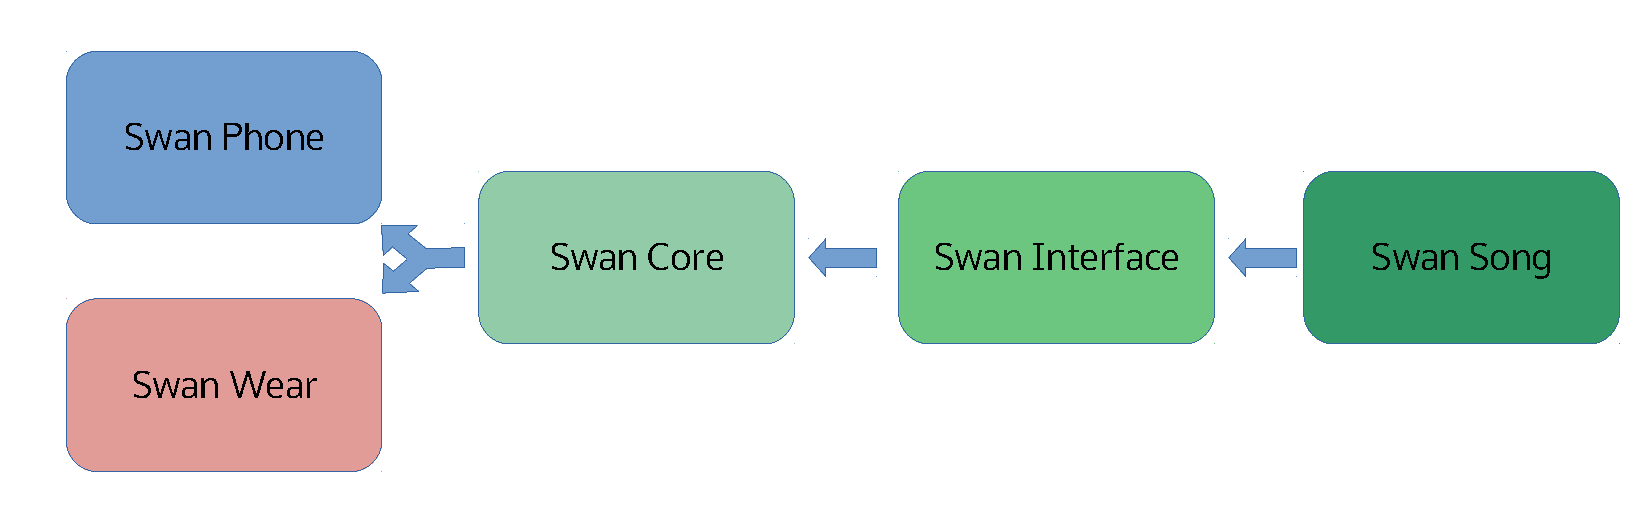
\includegraphics[scale=0.5]{Figures/swan_layout.pdf}
    \rule{35em}{0.5pt}
  \caption[SWAN Layout with separated libraries]{SWAN Layout with separated libraries}
  \label{fig:swan_layout}
\end{figure}

After SWAN Core was made independent, we decided to extract SWAN Song and SWAN Interface from it and make them separate libraries, as we can see in \hyperref[fig:swan_layout]{Figure 5.1}.
The main reason for this library separation was the way applications interact with SWAN. The SWAN Interface is often imported as a separate JAR in any application that wants to register a 
SWAN expression. To improve the distribution of the Swan Interface, we decided to make it available\footnotemark  on Android Main Repository - JCenter\cite{jcenter}. 
\footnotetext{Uploading the JARS required us to follow the tutorial by The Cheese Factory\cite{jcenter_tutorial}.}

Because we are maintaining the packages on JCenter now, the old packages and package building scripts  in the repository were discarded.
The JCenter  is not storing the packages in JAR format, but in the new format made to accommodate the Android Resources: AAR \cite{aar_format}. 
The new package format can be built and uploaded directly from Android Studio. 

More information about how to manage and upload the SWAN libraries is available on SWAN wiki's Github\cite{swanWiki}.

\subsection{SWAN On Android Wear}
When compared to initial SWAN application, SWAN on Android Wear, or mini-SWAN is only a part of the original application.
The list of components that are not included in mini-SWAN:
\begin{itemize}
 \item Proximity Manager - This component is not relevant for smartwatch. We do not intend to further forward the expression.
 \item Configuration Activity - We only implement an evaluation service with no UI components
 \item Beacon Discovery - While smartwatch has scanning capabilities, it is better to leave this component for phones
 \item Database storage - The space on the watch is limited and we are only interested in forwarding values
\end{itemize}

Compared to normal SWAN expression, a wear expression has the \hyperref[fig:SwanExpression]{location string} set to \textbf{wear} keyword. Evaluation Engine is responsible for changing the location
to \textbf{self} and forwarding the expression to SWAN on the smartwatch.
The implementation of expression based smartwatch sensors added on top of the existing value based implementation. New commands were added to start and stop a SWAN expression on the watch.
The values sent back use the same implementation as for value based sensors.

\section{Difference between Value Based And Expression Based Sensors}
Value Based sensors will send all the values from the smartwatch to the phone. In some particular cases, not all values will be accepted by the SWAN.
Sending too many values over Bluetooth will impact battery life on both devices.
Expression based sensors will evaluate the values locally, on the watch, and only send the result over Bluetooth. On the other hand, performing
computations on the watch can impact battery life. Still, expression based offers very low power consumption on the phone, as we can see from the power analysis in \hyperref[Chapter6]{Chapter 6}.
